%************************************************
\chapter{Discussion}
\label{chp:Discussion}
%************************************************
%\section{Parallel processing streams and their functional significance}
%Parallel processing seems to be a successful evolutionary strategy conserved throughout phyla. Other than the visual system, the olfactory system of the nematode C elegans \parencite{Chalasani2007} and the auditory cortex of mammals \parencite{Scholl2010} are some examples where parallel circuits compute ON and OFF signals separately. 
\section{Comparison between ON and OFF pathways in the fly optic lobe and the mouse retina}
Among the most striking similarities between the retina and the fly optic lobe is the early splitting of pathways into ON and OFF channels (figure \ref{fig:flymouse}). This allows for more efficient encoding of visual stimuli \parencite{Gjorgjieva2014}. In the vertebrate retina, this splitting takes place right at the photoreceptor-bipolar synapse, but in the fly, it occurs one synapse later.

In the mouse retina, in the dark, photoreceptors release glutamate into their postsynaptic partners, the bipolar cells. In response to light, photoreceptors hyperpolarize. There are ON and OFF responsive bipolar cells. In ON bipolar cells, the metabotropic inhibitory glutamate receptor mGluR6 causes a sign inversion and the ON channel is formed \parencite{Masu1995}. The OFF bipolar cells, however, express ionotropic AMPA receptors that depolarize when glutamate binds \parencite{Euler2014}. As in the fly optic lobe, there are fast and slow bipolar cells, similar to the medulla and transmedulla neurons.

The split into ON and OFF pathway occurs at the level of lamina cells in the fly. Vertebrates don't seem to have any equivalent to the lamina. \textit{Drosophila} photoreceptors depolarize under light and release histamine, which in turn inhibits lamina neurons via histamine-gated chloride channels \parencite{Hardie1989}. Cholinergic lamina neurons L2-L5 transmit photoreceptor signals to medulla and transmedulla neurons. In the ON channel, L1 is the main input, while in the OFF channel, L2 is the main input \parencite{Joesch2010}. The glutamatergic L1 neurons inhibit postsynaptic Mi1 and Tm3 neurons via the glutamate-gated chloride channel GluCl$\alpha$, implementing a sign inversion and creating an ON channel. Thus, photoreceptors depolarize in response to light, inhibiting L1 neurons, thereby disinhibiting Mi1 and Tm3 neurons, creating ON-responses. Both GluCla and Rdl receptors are involved in this multi-synaptic sign inversion in the ON pathway \parencite{Molina2019}. Both mouse and fly visual systems exhibit sign inversion in the ON pathway as a result of glutamatergic, inhibitory signaling. Fly uses the GluCl$\alpha$ channel, which is unique to invertebrates, instead of the mGluR6 receptor, which causes inhibition in the mouse retina.

Direction-selective T4/T5 cells in flies are comparable to starburst amacrine cells (SACs) in mammals and lobula plate tangential cells are comparable to direction-selective ganglion cells (figure \ref{fig:flymouse}).
\begin{figure}
\centering
\hspace*{-1cm} 
\includegraphics[scale=0.6]{fly_mouse_comparison}
\caption[Fly and mouse motion detection circuits] {Fly and mouse motion detection circuits: In the fly, the photoreceptors connect via sign-inverting synapses to lamina monopolar cells L1 and L2, the entry to the ON and OFF pathway, respectively. The mouse retina lacks this additional layer of lamina cells and splits the signal directly between ON and OFF bipolar cells via two types of glutamate receptors. T4 (ON) and T5 (OFF) neurons in the fly optic lobe and ON and OFF SACs in the mouse retina are the first stage of direction-selective cells. Lobula plate tangential cells (LPTCs) in the fly and ON-OFF direction-selective ganglion cells (DSGCs) in the mouse integrate direction-selective information from these two pathways. (Used with permission from \cite{Borst2015})} 
\label{fig:flymouse}
\end{figure}
\section{Neural algorithm underlying direction selectivity}
Different models have been proposed to explain the neural computations involved in motion detection. In order to detect motion in a directionally selective manner, local motion detection mechanisms must meet certain minimum requirements \parencite{Borst1989}:
\begin{enumerate}
\item Spatial offset: Motion is a vector that needs two points to be represented, so at least two spatially separated inputs are required.
\item Temporal asymmetry: There must be at least one input that is delayed. If not, the input signals arrive in the subsequent stage simultaneously independent of the stimulus direction.
\item Non-linear interaction: It is necessary to integrate input signals nonlinearly at a subsequent stage of the process. In the absence of this, the detector's output would be equal for both directions on average.
\end{enumerate} 

Classically two opposing models have been proposed for implementation of direction selectivity. Both these model use two input lines, where one of the input line has been asymmetrically delayed compared to the other, which is then followed by a non-linear interaction. The Hassenstein-Reichardt (HR) model proposes a Preferred Direction (PD) enhancement: the signal on the preferred side is delayed and is subsequently amplified using multiplication of the signal from the other input line (figure \ref{fig:hrblmodel}a) \parencite{Hassenstein1956}. The Barlow-Levick (BL) detector however, proposes a Null Direction (ND) suppression: the signal on the null side is delayed and divides the signal from the other input resulting in suppression (figure \ref{fig:hrblmodel}b) \parencite{Barlow1965}. \cite{Haag2016} used apparent motion stimuli to show that both the mechanisms i.e. PD enhancement and ND suppression is used by T4 and T5 cell to produce a direction selective response (figure \ref{fig:hrblmodel}c). In the first manuscript \ref{sct:manuscript_haag_mishra} - \parencite{Haag2017}, we showed that all four subtypes of T4 and T5 indeed uses both PD enhancement and ND suppression to produce direction selective responses. Therefore, a new model combining both PD enhancement on the preferred side and ND suppression on the null side was proposed. The next important task now is to identify neural correlates implementing these mechanisms. 

The model requires a fast input at the center, slow input providing excitation on the preferred side and slow input providing suppression on the null side. Interestingly, from the anatomical and functional characterization of input data we have discussed earlier, we could predict the input neurons for T4 providing these three kind of inputs. Mi1 is a fast neuron providing input at the central part of dendrite, thus a candidate for central fast input. Mi9 is a slow neuron providing input on the preferred side of the dendrite, hence a candidate for slow excitatory input. Mi4, C3 and CT1 are slow neurons providing input on the null side of the dendrite. 

In addition to synaptic mechanisms on the dendrites of T4 cells, further processing in the T4 neurons can enhance the direction selectivity of the output signals. Neuronal signaling and information processing involves the transformation of membrane voltage into calcium signals, which lead to transmitter release. Computations can occur at different stages in the signaling cascade: 1.) dendritic integration and processing of voltage signals. 2.) transformation from voltage to calcium and 3.) between calcium and neurotransmitter release. In the second manuscript \ref{sct:manuscript_mishra_haag}, we explored the transformation of voltage to calcium in T4-cells. We found that the voltage to calcium transformation in T4c neurons enhances their direction selectivity: calcium signals in T4c cells have a significantly higher direction selectivity and tuning compared to membrane voltage across different stimuli conditions. 
\begin{figure}
\centering
\hspace*{-1cm} 
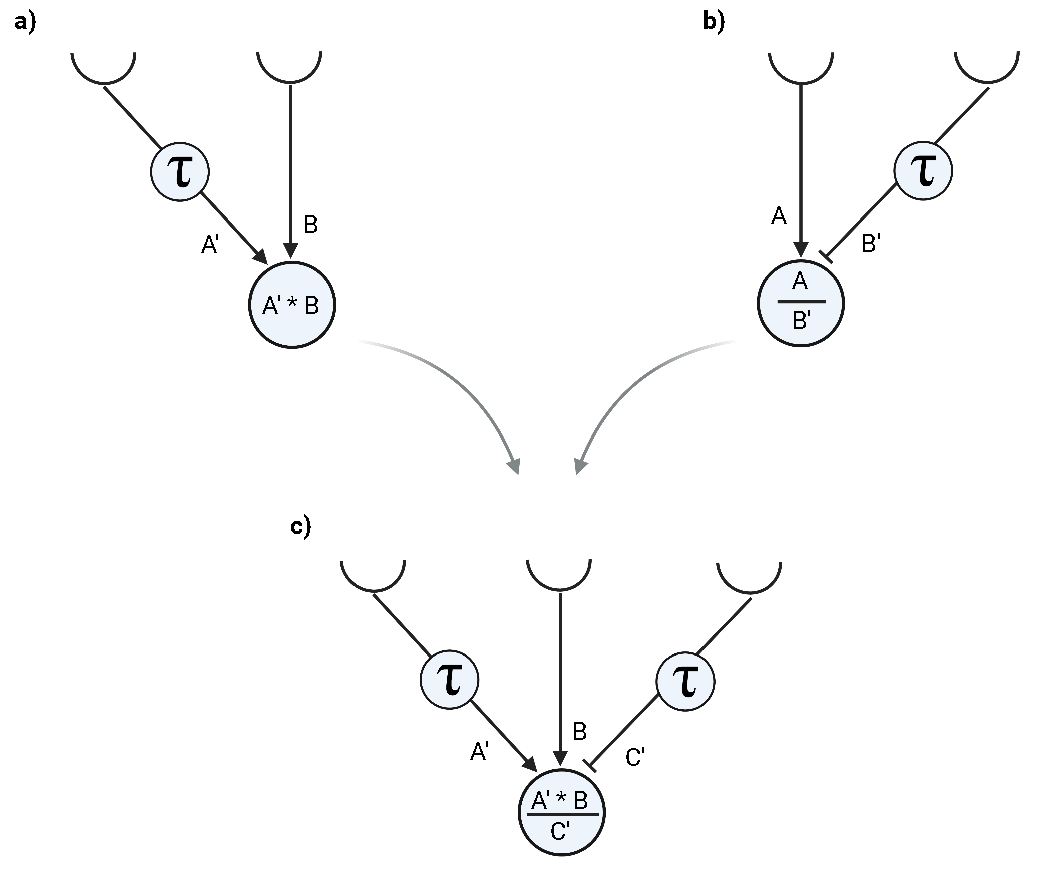
\includegraphics[scale=0.8]{HRBL_model}
\caption[Models for motion detection] {Models for motion detection: (a) The Hassenstein-Reichardt (HR) correlator (half-detector shown here) consists of two arms. Motion in the preferred direction (PD) causes two signals from neighboring photoreceptors to coincide due to a delay ($\tau$) on the first arm. There is an enhancement in PD resulting from a multiplicative non-linearity. (b) The Barlow-Levick (BL) detector has the delay on the opposite arm, and the non-linearity is inhibitory, resulting in a null-direction (ND) suppression. (c) Hybrid detector consisting of one HR unit and one BL unit: Three points in space are sampled. There is a time delay ($\tau$) on the outer two arms. The input signals from the detector arms A and B are multiplied and divided by the signal from the detector arm C in the following stage. Consequemtly, the signal in the preferred direction is enhanced and the signal in the null direction is suppressed.}
\label{fig:hrblmodel}
\end{figure}
\section{Effect of voltage to calcium transformation on T4 output signals}
In addition to the dendritic integration of postsynaptic voltages or after the action potential is generated, further computations can occur in the transformation between voltage and calcium, or between calcium and neurotransmitter release. Neuronal signaling and information processing involves the transformation of membrane voltage into calcium signals, which lead to transmitter release. In our second manuscript \ref{sct:manuscript_mishra_haag}, we showed that voltage to calcium transformation in T4c neurons enhances their direction selectivity. The calcium signals in T4c cells had a significantly higher direction selectivity and tuning compared to membrane voltage across different stimuli conditions. The direction selectivity index for calcium signals compared with voltage signals for a few stimuli conditions was previously found to be higher in a study in T5 cells using ASAP2f as an optical voltage indicator \parencite{Wienecke2018}. How does this affects the output signal of T4/T5 neurons?

As calcium is required for neurotransmitter release, this is expected to increase the direction selectivity of T4/T5 cells' output signals. In the lobula plate, T4/T5 cells provide inputs onto large lobula plate tangential cells that are depolarized during preferred and hyperpolarized during null direction motion \parencite{Mauss2014}. For example, vertical system (VS) cells with dendrites in layer 4 receive direct excitatory inputs from downward tuned T4d/T5d neurons causing depolarization during motion in the downward preferred direction. These VS cells also receive indirect inhibitory inputs from upward tuned T4c/T5c neurons via glutamatergic LPi3-4 neurons projecting from layer 3 to layer 4 causing hyperpolarization in VS cells during motion in the upward null direction. Upon silencing LPi3-4 neurons’ synaptic output via tetanus toxin, VS neurons depolarization response in the preferred direction did not change, but the null direction response was absent \parencite{Mauss2015}. This suggests T4/T5 do not release any transmitter in response to null direction motion, which matches our findings for the calcium responses. Thus, voltage to calcium transformation increases direction selectivity in T4/T5 cells and this enhances direction selectivity in downstream neurons. 

\section{Differential expression of voltage-gated calcium channels}

In manuscript \ref{sct:manuscript_mishra_haag}, we built a model to capture voltage to calcium transformation in T4c, Mi1, and Tm3 cells. A simple model with a single low-pass filter was able to reproduce calcium responses in non-direction-selective Mi1 and Tm3 cells, whereas a more complex model combining the output of two low-pass filters via a multiplication was required to reproduce T4c calcium responses. The direction selectivity for the simple model signals for T4c was lower compared to the multiplicative model. This suggests that voltage-calcium transformation in Mi1 and Tm3 cells is different from those in T4c cells. 

Differential expression of voltage-gated calcium channels in these cells could explain the different voltage to calcium transformation. Voltage-gated calcium channels mediate depolarization-induced calcium influx that drives the release of neurotransmitters. The $\alpha1$-subunit of the voltage-gated calcium channels forms the ion-conducting pore, which makes it distinct from other calcium channels. Three families of genes encode $\alpha1$ subunits. \textit{Drosophila} genome has one $\alpha1$ subunit gene in each family: $\alpha1D$ ($Ca_{v}1$), cac ($Ca_{v}2$), and $\alpha1T$ ($Ca_{v}3$) \parencite{Littleton2000, King2007}. In \textit{Drosophila} antennal lobe projection neurons, cac ($Ca_{v}2$) type and $\alpha1T$ ($Ca_{v}3$) type voltage-gated calcium channels are involved in sustained and transient calcium currents, respectively \parencite{Gu2009, Iniguez2013}. According to a RNA-sequencing study \parencite{Davis2020}, $\alpha1T$ ($Ca_{v}3$) mRNA have higher expression in Mi1 ($2050.16$ Transcripts per Million (TPM)) compared to T4 ($686.68$ TPM) and Tm3 ($336.45$ TPM). While cac ($Ca_{v}2$) mRNA have higher expression in T4 ($1298.53$ TPM) compared to Mi1 ($986.25$ TPM) and Tm3 ($817.61$ TPM). Different expression of voltage-gated calcium channels could cause different voltage to calcium transformations in non-direction selective and direction-selective cells.

\section{Conclusion}
In the course of this work, I investigated neural computation in the \textit{Drosophila} motion vision pathway. Together with my co-authors, we showed that both preferred direction enhancement and null direction suppression are implemented in all four subtypes of T4 and T5 cells. Already at the first stage of direction selectivity computation, this combined strategy ensures a high degree of direction selectivity. Additionally, we showed that voltage-to-calcium transformations further enhance direction selectivity in the output signals of T4 cells in addition to the synaptic mechanisms at the dendrites. We built a model to transform voltage signals into calcium signals. The model was more complex for direction-selective T4 cells compared to non-direction selective cells Mi1 and Tm3. Future work will focus on comparison of voltage-gated calcium channels in these neurons which lead to different voltage to calcium transformation.



